%\section {Data Analysis on \NAME}
\section {Analyzing Aggregated Results}\label{Analysis}

Since prior works only focus on the design of SQL evaluated over encrypted data,
the capability of further data processing on the queried result is mostly left 
unexplored. Here, we first discuss how to efficiently bridge the gap between 
the database query and online data analysis, and then show
a case study using private decision tree evaluation.
% sortinghat 
% Main point: existing data analysis methods may not achieve the best efficiency
% when dealing with database results

\subsection{Bridging DB Aggregation and Data Analysis}\label{Analysis: Bridge}
%Statistical Data Analysis}
\begin{figure}[t!]
   \begin{center}
   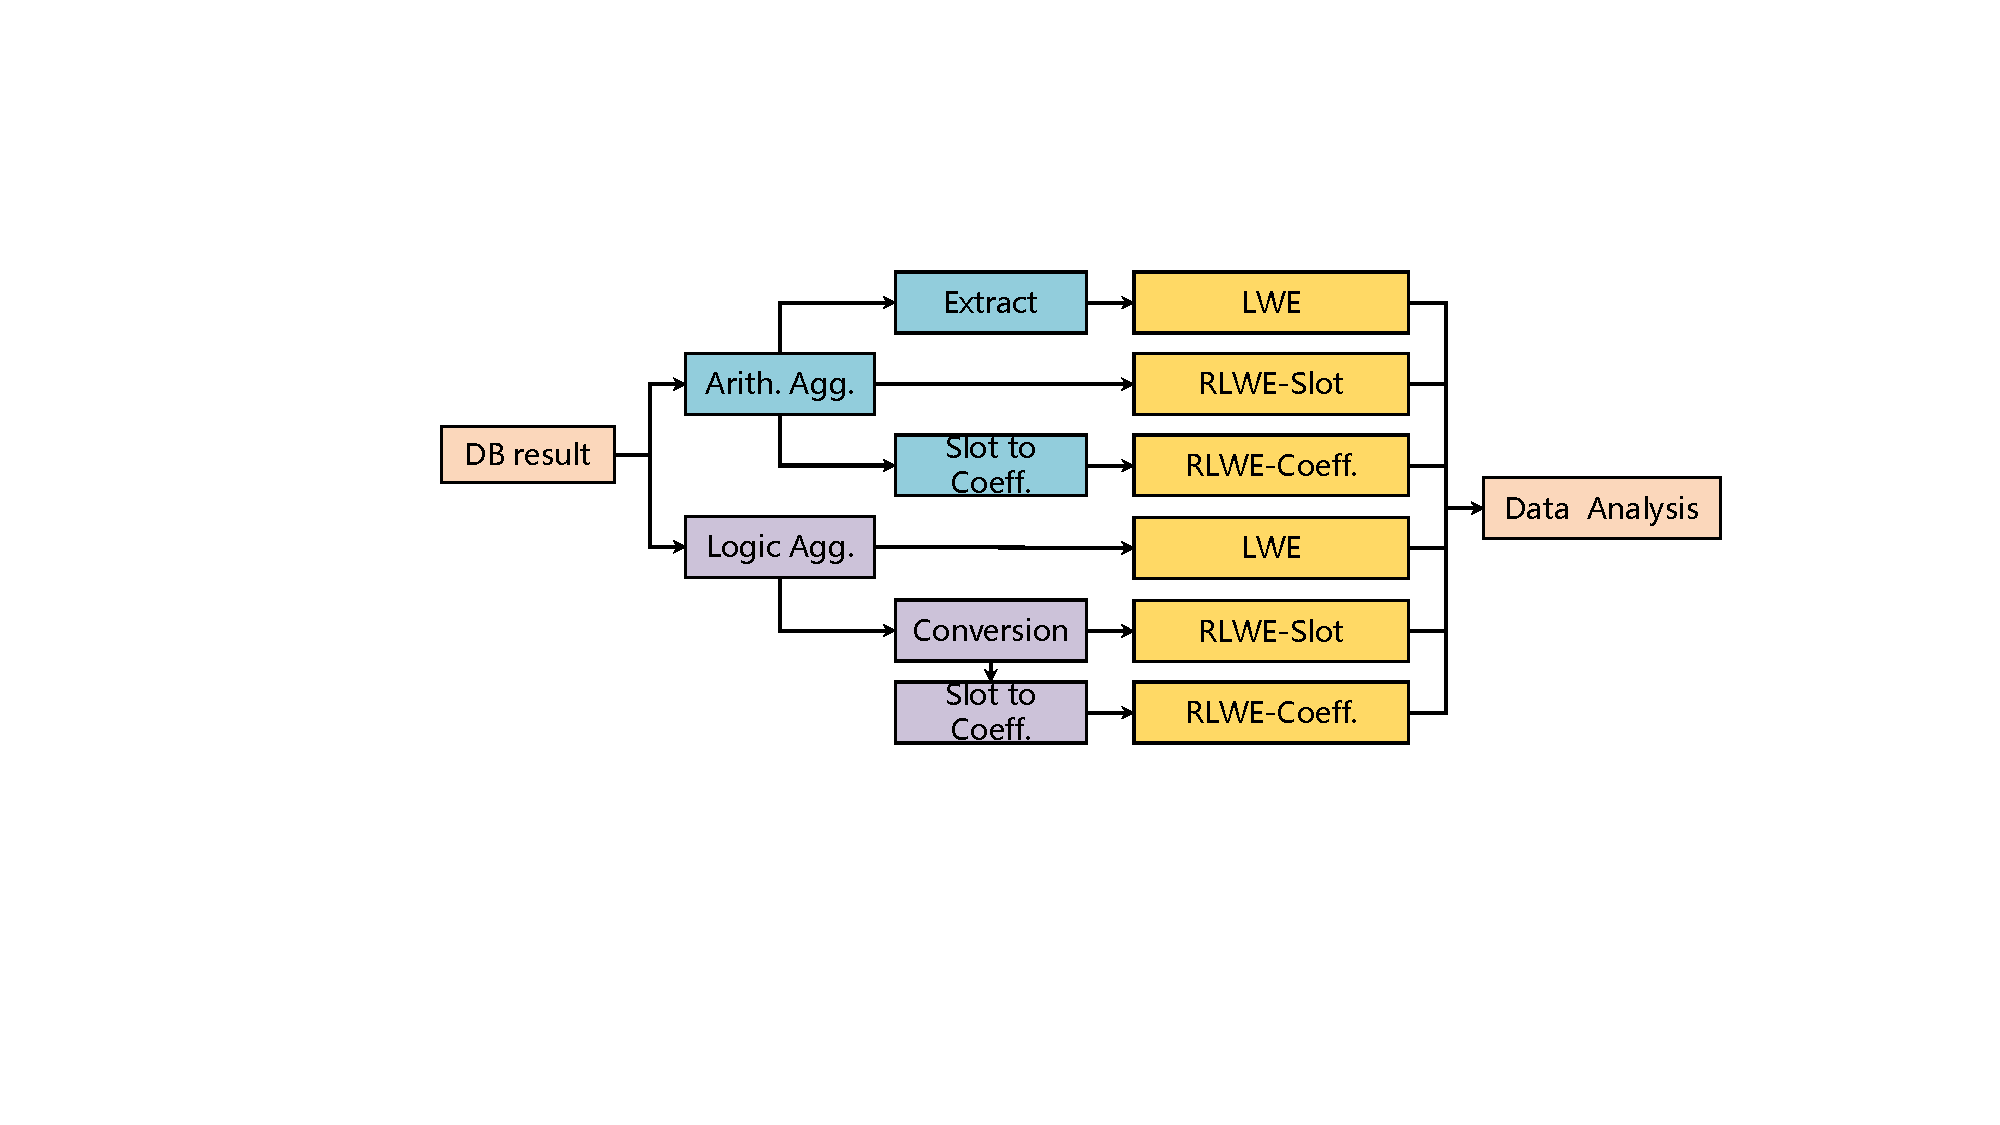
\includegraphics[width=\linewidth]{figure/conversion.pdf}
   \end{center}
    % \vspace{-0.5em}
      \caption{The conversion procedures to turn
      the aggregation results into data analysis inputs.} 
      \Description{Figure 4. Fully described in the text.}
   \label{fig: bridge}
   % \vspace{-0.5em}
\end{figure}

As shown in \cref{fig: bridge}, to support efficient data analysis algorithms
using both arithmetic and logic operators, we need to convert the queried
results into three different ciphertext formats: an LWE ciphertext ($\lwe$),
an RLWE ciphertext with slot encoding ($\rlweslot$), and an RLWE ciphertext
with coefficient encoding ($\rlwecoeff$).
% In order to evaluate general data analysis application which contains both
% arithmetic and logic circuits without client-server interactions,
% we summarize a bridging mechanism of 
% the arithmetic and logic aggregation result into 
% three different types of data analysis input in \cref{fig: bridge}.

% \textbf{Results from Logic Aggregation}: 
We first discuss the conversion algorithms for logic aggregations.
Note that, logic aggregation produces LWE ciphertexts as results. Therefore,
as sketched in \cref{fig: bridge}, there is no need of conversion if
the subsequent data analysis algorithm acts on LWE ciphertexts. For
other formats of ciphertexts, the following operators can be applied.
% and can be
% converted into other formats by the following operators.
% $\bullet$ \textbf{To LWE}: the logic aggregation results could be 
%     naturally applied to the data analysis application in the case of 
%     single value single data (SISD). 

$\bullet$ To $\rlweslot$: %\textbf{To $\rlweslot$}: 
Converting a set of LWE ciphertexts into an 
RLWE ciphertext in slot representation is precisely the proposed
$\repack$ operator described in \cref{block: LWEsPack}.

$\bullet$ To $\rlwecoeff$: %\textbf{To $\rlwecoeff$}: 
    Convert between the slot and coefficient forms for an RLWE ciphertext
    is well-studied in existing 
    literature~\cite{DBLP:journals/access/s2cc2s, betterboot, improvedboot, inverseboot}. 
    Thus, converting multiple $\lwe$ ciphertexts into an $\rlwecoeff$ ciphertext
    can be constructed by first applying the $\repack$ operator followed
    by the slot-to-coefficient transform.
%\end{itemize}

% \textbf{Results from Arithmetic Aggregation}: 
%\paragraph{Results from Arithmetic Aggregation}
Different from logic aggregations, the arithmetic aggregation results 
are RLWE ciphertexts in the 
slot representation. Hence, we can apply the following conversions to
the resulting ciphertext for subsequent data processing.
%\begin{itemize}

$\bullet$ To $\lwe$: %\textbf{To $\lwe$}: 
We can simply apply $\sei$ to
extract LWE ciphertexts from an RLWE ciphertext.
%     needs to first change the slot representation to the coefficient 
%     representation \texttt{CoeffToSlot}
%     and sample extracts the LWE ciphertexts.
% \textbf{To RLWE-Slot}: the arithmetic aggregation results could be 
%     naturally applied to the data analysis application in the case of 
%     single value multiple data (SIMD). 

$\bullet$ To $\rlwecoeff$: We can simply apply
the slot-to-coefficient transform above to convert 
$\rlweslot$ into $\rlwecoeff$~\cite{DBLP:journals/access/s2cc2s}.
% to fit some cases where coefficient 
% representation is more efficient in data analysis.
%\end{itemize}

% The arithmetic aggregation basically follows the 
% slot representation of RLWE ciphertext.


% As the LWE ciphertext 
% ciphertexts types, such as that between coefficient and slot
% representations~\cite{DBLP:journals/access/s2cc2s} 
% and that between SIMD and SISD 
% representations~\cite{DBLP:conf/sp/pegasus,DBLP:conf/acns/conversion}.
% There are three types of HE ciphertexts used in data analysis:
% LWE ciphertext, which is frequently used in SISD 

% \textbf{Logic Aggregation}: 

%{\bf{Private Decision Tree over Aggregated Results}}:
\subsection{Case Study: Private Decision Tree}\label{Analysis: PDTE}
Here, we take private decision tree evaluation (PDTE) as an example to combine the 
evaluation flows of \NAME.
A PDTE algorithm~\cite{sortinghat, pegasus} basically implements the following function 
over a set of LWE ciphertexts.
\begin{equation}
%(\lwe_{{\rm o}, 0}, \cdots, \lwe_{{\rm o}, \ell-1}) = \pdte(\lwe_{{\rm i}, 0}, \cdots, \lwe_{{\rm i}, d-1}, \algoweight),
\{\lwe_{{\rm output}, i}\}= \pdte(\{\lwe_{{\rm input}, j}\}, \algoweight),
\label{eq:pdte_conv}
\end{equation}
where a set of ciphertext inputs $\{\lwe_{{\rm input}, i}\}$ are
classified into $\ell$ output
ciphertext classes $\{\lwe_{{\rm output}, j}\}$ based on the pre-trained parameters $\algoweight$. 
Similar to existing works~\cite{sortinghat}, inputs and outputs of $\pdte$ are all LWE 
ciphertexts, since the evaluations of decision
trees consist mostly of non-linear operations. As mentioned,
we have two possible formats of ciphertext after the evaluation of an SQL query 
with aggregation: $\lwe$ and $\rlweslot$. Since logic aggregation naturally produces
an $\lwe$ ciphertext, the output can directly be fed into a PDTE algorithm. Meanwhile,
if we need to carry out PDTE over the arithmetically aggregated results, we can
simply apply $\sei$, as described in \cref{Analysis: Bridge}, and proceed with
the evaluation of \cref{eq:pdte_conv}. %Eq.~\eqref{eq:pdte_conv}. 

{\bf{Remark}}: Since most existing FHE-based PDTE algorithms are designed for 
two-party secure computing~\cite{pegasus, sortinghat}, the model parameters 
$\algoweight$ in \cref{eq:pdte_conv} are assumed to be known to the server. 
However, such an assumption does not always hold true in SDO, where the
data analysis algorithm can also be 
outsourced~\cite{shan2018practical,matsuoka2021virtual}. In particular,
switching PDTE to a computation outsourcing setting actually requires a complete
re-design of the evaluation protocol. Due to space limitation, we provide a complete 
description of our proposed SDO-orient PDTE algorithm based on the proposed
$\homcomp$ operator in the Appendix.

%A decision tree is a binary tree structure with a set of decision nodes and leaf nodes. It implements a mapping $\textbf{F}: \mathbb{Z}_{n}\rightarrow \{{w_0},...,{w_{\mathfrak{d}-1}}\}$, that maps an attribute vector $\mathbf{x} = ({x_0},...,{x_{n-1}})$ to a finite set of classification labels $\{{w_0},...,{w_{\mathfrak{d}-1}}\}$. The $i$-th decision node has threshold value ${t}_{i}$ and attribute index ${a}_{i}$ , while the $i$-th leaf node has label value ${w}_{i}$. Given a decision tree, the index of a node is its order as computed by breadth-first traversal, starting at the root with index 0. We denote $\mathfrak{d}$ as number of leaf nodes. If the tree is complete, the number of decision nodes is $\mathfrak{d} - 1$.

%The private decision tree is an encrypted version of the decision tree. After query processing, the server gets an aggregation result  $\mathcal{CR}$ = $(cr_0, cr_1,..., cr_{\lvert G \rvert})$ and client performs model encryption to obtain the private decision tree model $\mathcal{CM}$. During model encryption,  each threshold value $t_i$ is encrypted as $ct_i$, while each label value $w_i$ is encrypted as $cw_i$. Then the client sent the encrypted model $\mathcal{CM}$ to the server.

% Before Model Evaluation, the result of aggregation and the input of data analysis needs to be bridged through the function described in above. In the case of private decision tree, conventional technique \cite{sortinghat} \cite{pegasus} takes LWE ciphertexts as input, because the main operation in evaluating private decision tree is logic operation such as comparison. However, existing methods only useful under SQE model, and cannot be implemented in SDO model, because they require the decision tree parameters to be plaintext. Therefore, as an independent contribution, we propose a private decision tree evaluation algorithm \pdte, detailed in \cref{algo:pdte}, which can performs subsequent data analysis over both inputs and model parameters are encrypted.

%In \cref{eva:pdte}, we demonstrate that our \pdte function achieves 12x to 326x better evaluation time on different datasets and input size compared with existing work \cite{sortinghat}.


% As the output of logic aggregation and arithmetic aggregation
% may be distinct ciphertext formats.

% dimension lifting 
% The \texttt{LWEsPack} reaches good performance in the pack of 
% a lot of LWE ciphertexts.
% We aim to design an efficient 
% dimension-lifting \texttt{LWEToRLWE} algorithm
% that only performs one LWE ciphertext to an RLWE ciphertext. 
% Existing work ~\cite{conversionhaochen}

% Particularly, Chen~\cite{conversionhaochen} recently presented 
% a key-switching algorithm for LWE ciphertexts of 
% the same lattice dimension. 
% PEGASUS~\cite{pegasus} modify their algorithm for the dimension n > n. 
% We consider the case of dimension n < n 
% and propose a general dimension-switching algorithm.
\begin{table}[t!] 
    \centering
    \caption{The Proposed Parameter Sets}
    \vspace{0em}
        \begin{tabular}{cc}
            \toprule
            Ciphertext &  Parameters\\
            \midrule
            LWE & $n=672, \upint{\log_{2}{q} } = 32$\\
            RLWE & $N=65536, \upint{\log_{2}{Q} } = 653$\\
            RGSW & $N'=2048, \upint{\log_{2}{Q'} } = 64$\\
            % \multirow{3}*{LWE} & $n = 672, sd = 2^{-16}, 
            % \upint{\log_{2}{q} } = 32$ \\
            % & $n = 1024, sd = 2^{-25}, 
            % \upint{\log_{2}{q}} = 32$ \\
            % & $n = 2048, sd = 2^{-52}, 
            % \upint{\log_{2}{q}} = 64$ \\
            % \multirow{2}*{RWE} & $n = 1024, sd = 2^{-16}, 
            % \upint{\log_{2}{q} } = 32$ \\
            % & $n = 65536, \sigma = 3.19, 
            % \upint{\log_{2}{q_i} } = 32$ \\

            \bottomrule
        \end{tabular}
    \label{tab:parameters}
    % \vspace{-3mm}
\end{table}
\begin{table*}[t!] 
    \centering
    \caption{Qualitative Comparisons Between Homomorphic Comparison Algorithms}
    % \vspace{-0.5em}
        \begin{tabular}{cccccccc}
            \toprule
            & Kortekaas~\cite{aphadb}
            & Antonio \etal~\cite{revisiting}
            & Pegasus~\cite{pegasus} 
            & Liu \etal~\cite{largeprecision}
            & SortingHat~\cite{sortinghat} 
            & Cheon \etal~\cite{ckkscomparison} 
            & Ours\\
            \midrule
            Cipher-cipher comp.$^{+}$ & \yeah & \yeah & \yeah & \yeah & \nope & \yeah& \eyeah \\
            Full comparison & \yeah & \noyeah$^{++}$ & \yeah & \yeah & \yeah & \noyeah$^{++}$& \eyeah \\
            %16bit-precision & \yeah & \yeah & \nope & \yeah & \yeah & \yeah & \eyeah \\
            32-bit precision & \yeah & \yeah & \nope & \nope & \yeah & \nope & \eyeah \\
            %Predicate evaluation & \yeah & \nope & \yeah & \yeah & \yeah & \yeah & \eyeah \\
            Unbounded depth & \nope & \nope & \yeah & \yeah & \yeah & \nope & \eyeah\\
            Flexible parameter. & \noyeah$^{*}$ & \nope & \yeah & \nope & \nope & \noyeah$^{*}$ & \eyeah\\
            Efficiency & High & High & Low & Low & Low & High & High\\
            Storage & High & High & Low & Low & High & High & Low\\
            \bottomrule
        \end{tabular} \\
        {
        \footnotesize{
        %\begin{flushleft}
        $^{+}$Cipher-cipher comparison refers to the case where both of the 
        inputs to the comparison function are ciphertexts \\
        $^{*}$Changing encryption parameters requires the re-encryption the database 
        $^{++}$Do not support encrypted aggregations over results
        from equality comparison
        %\end{flushleft}
        }}
    \label{tab:homcom}
    % \vspace{-3mm}
\end{table*}